\section{Background}
\label{sec:background}
%

%
\subsection{Transformer-based LLMs and their Limitations}
\label{subsec:background_llm}
%
\begin{figure}[t]
  \centering
  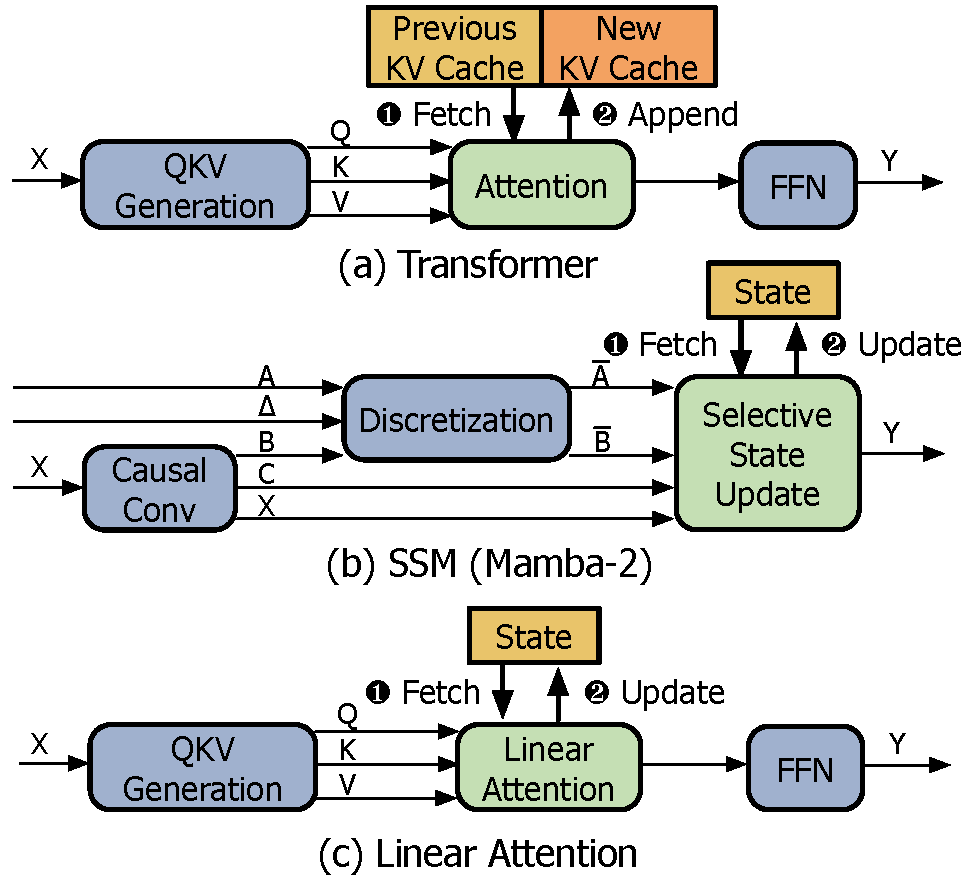
\includegraphics[width=0.8\linewidth]{fig/LLM.pdf}
  \caption{Model architectures of (a) Transformer, (b) Mamba-2 of
    SSM, and (c) Linear Attention. For simplicity, we focus on the
    key operations.
  }
  \label{fig:LLM}
\end{figure}
%
\niparagraph{Transformer-based LLMs.}
%
Transformers offer remarkable performance due to their attention
mechanism, which enables efficient modeling of inter-token
dependencies~\cite{llama2, devlin2019bert, Rub1, Rub2}.
%
Figure~\ref{fig:LLM}(a) shows the model architecture for transformer-based LLMs.
%
In the attention mechanism, each token in the input sequence is
projected into three distinct vectors: query ($Q$), key ($K$), and value ($V$).
%
The query and key vectors are used to compute the attention scores by
taking the scaled dot product, and the value vectors are used to
perform a weighted sum over these scores.
%

%
\niparagraph{Limitations.}
%
The auto-regressive nature of LLM requires revisiting all previous
tokens, resulting in redundant computation.
%
Key-Value (KV) cache is employed to prevent recomputing previous
tokens, but the transformers face the following limitations:
%

%
\aptLtoX{\begin{itemize}
  \item[(1)] \textbf{Memory usage.}
     The KV cache grows linearly with the sequence length. Despite
    prior work on enhancing memory
    efficiency~\cite{hooper2024kvquant, yang2024token, dong2024qaq,
    kang2024gear,vllm}, the fundamental property of the algorithm is
    unchanged. This ends up consuming significant amounts of GPU
    memory and imposing limits on the sequence length or the batch size.
    \item[(2)] \textbf{Latency.}
    The computation of attention layers increases linearly, even with
    the KV cache, leading to increased latency with longer sequences.
    %
    In multi-user serving scenarios, typically processed in batches,
    the difference in compute latency can hinder efficient
    scheduling~\cite{orca,vllm}.
    %
\end{itemize}}{\begin{description}[labelindent=0.0em,nolistsep,leftmargin=1.5em]
    %
  \item[(1)] \textbf{Memory usage.}
    %
    The KV cache grows linearly with the sequence length. Despite
    prior work on enhancing memory
    efficiency~\cite{hooper2024kvquant, yang2024token, dong2024qaq,
    kang2024gear,vllm}, the fundamental property of the algorithm is
    unchanged. This ends up consuming significant amounts of GPU
    memory and imposing limits on the sequence length or the batch size.
    %

  \item[(2)] \textbf{Latency.}
    %
    The computation of attention layers increases linearly, even with
    the KV cache, leading to increased latency with longer sequences.
    %
    In multi-user serving scenarios, typically processed in batches,
    the difference in compute latency can hinder efficient
    scheduling~\cite{orca,vllm}.
    %
\end{description}}

%
\subsection{Post-Transformer LLMs}
\label{subsec:ssm_based_llms}
%
Recently, alternative architectures including state space models
(SSMs)~\cite{mamba, s4, h3, hyena, s4d, hippo, lssl, mamba2}, linear
attention mechanisms~\cite{retnet, linear_attention,
gated_linear_attention, gsa}, and recurrent neural networks
(RNNs)~\cite{hgrn2, rwkv, rwkv6, xlstm} have emerged as promising
substitutes for transformers.
%
These \emph{post-transformer} models offer comparable capabilities to
transformers, while requiring constant resources regardless of
sequence length, addressing the fundamental limitations of transformers.
%

%
\niparagraph{SSM.}
%
Among the alternatives, state space models (SSMs) have demonstrated
their effectiveness, leveraging structured state transitions to
efficiently capture long-range dependencies.
%
The state-of-the-art, Mamba-2~\cite{mamba2}, achieves leading
performance among SSMs through its selection mechanism that
efficiently propagates prior token information.
%
Given the prominence of Mamba-2 in language modeling and its adoption
in numerous new models~\cite{huang2024mlmamba,
nvidia-mamba2, zamba2, codestral}, this
paper focuses on Mamba-2 as a representative of SSMs.
%

%
Figure~\ref{fig:LLM}(b) illustrates the key operations of Mamba-2.
%
Among these, the selective state update operation is the core in
Mamba-2, which operates with $H$ parallel heads, akin to the
multi-head attention mechanism in transformers.
%
The inputs to the selective state update include vectors
$\overline{A}$, $\overline{B}$, $C$, and $X$.
%
These are partitioned across the $H$ heads, yielding scalar $a^h$ and
vectors $\overline{B^h}$, $C^h$, and $X^h$ for each head.
%
Each head maintains its own state matrix, which is updated through
the following steps at each time step:
%
\aptLtoX{\begin{itemize}%[labelindent=0.0em,nolistsep,leftmargin=1.5em]
    %
  \item[(1)] \textbf{State decay.} The previous state matrix is
    decayed by multiplying it with scalar $a^h$, decaying the
    influence of older information.
    %
  \item[(2)] \textbf{Outer product.} The outer product of vectors
    $\overline{B^h}$ and $X^h$ is computed, capturing the
    interactions between these vectors.
    %
  \item[(3)] \textbf{Update.} The resulting outer product matrix is
    added to the decayed state to form the updated state.
    %
  \item[(4)] \textbf{Output.} A GEMV operation between the updated
    then transposed state matrix and vector $C^h$ produces the output vector.
    %
\end{itemize}}{\begin{description}[labelindent=0.0em,nolistsep,leftmargin=1.5em]
    %
  \item[(1)] \textbf{State decay.} The previous state matrix is
    decayed by multiplying it with scalar $a^h$, decaying the
    influence of older information.
    %
  \item[(2)] \textbf{Outer product.} The outer product of vectors
    $\overline{B^h}$ and $X^h$ is computed, capturing the
    interactions between these vectors.
    %
  \item[(3)] \textbf{Update.} The resulting outer product matrix is
    added to the decayed state to form the updated state.
    %
  \item[(4)] \textbf{Output.} A GEMV operation between the updated
    then transposed state matrix and vector $C^h$ produces the output vector.
    %
\end{description}}
%

%
In this sequence, each head effectively updates its internal state
based on inputs, producing outputs that contribute to the model's
overall computation.
%

\begin{figure}[t]
  \centering
  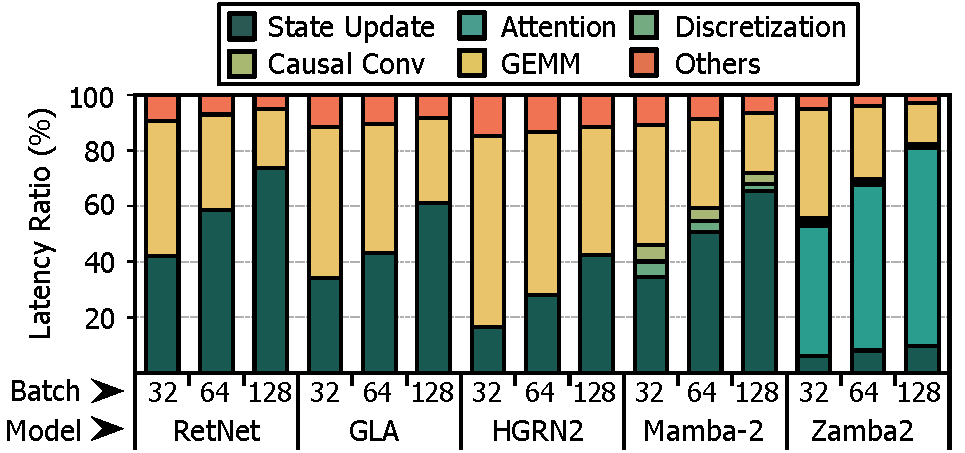
\includegraphics[width=\linewidth]{fig/motivation_breakdown.pdf}
  \caption{Latency breakdown of operations during generation phase on
    various SU-LLMs. For RetNet, GLA, HGRN2, and Mamba-2, we use a
    single generation phase due to their constant-time behavior. For
  Zamba2, we use (2,048, 2,048) input/output lengths.}
  \label{fig:motivation_breakdown}
\end{figure}

\niparagraph{Linear Attention.}
%
One approach is to propose entirely new architectures, such as SSM.
%
Alternatively, modifying the existing attention mechanism offers
another way to address the limitations of transformers.
%
Among such approaches, linear attention~\cite{linear_attention,
retnet, gated_linear_attention, gsa} has garnered significant
interest, as it replaces the softmax function in attention with a
linear function.
%
Since most linear attention mechanisms use the identity function as
the linear function, it can be expressed as
Equation~\ref{eq:linear_attention} and is illustrated in
Figure~\ref{fig:LLM}(c).
%
\begin{equation}
  LinearAttention(Q, K, V) = Q \cdot (K^T \cdot V)
  \label{eq:linear_attention}
\end{equation}
%
During the generation phase, the $K^T \cdot V$ product is used as the
state, which is continuously updated.
%
This is a constant-size state that does not grow with sequence length
and corresponds to steps (2)-(3) of the selective state update
operations in SSMs.
%
Multiplication of the state with $Q$ corresponds to the final step (4).
%
When a scalar decay factor is applied (e.g., RetNet~\cite{retnet}),
the linear attention mechanism aligns with the selective state update
operation in Mamba-2.
%
Conversely, applying an input-dependent gating mechanism (e.g.,
GLA~\cite{gated_linear_attention}) replaces the scalar decay factor
with a gating vector, which is broadcast and multiplied element-wise
with the state.
%
In short, both RetNet and GLA share the same or very similar state
update operation as Mamba-2.
%

\niparagraph{RNN.}
%
RNNs are being actively revisited as an alternative to transformers
for their linear computational complexity~\cite{rwkv, rwkv6, hgrn2, xlstm}.
%
Among these, HGRN2~\cite{hgrn2} introduces a novel architecture by
extending the conventional RNN state representation from a
one-dimensional to a two-dimensional state using an outer
product-based approach.
%
Interestingly, this operation closely resembles step (2) of the
selective state updates.
%
The forget gate in HGRN2 functions similarly to the decay mechanism,
while it employs a forget gate vector instead of a decaying scalar, akin to GLA.
%

%
\niparagraph{Combining with attention.}
%
Although aforementioned architectures demonstrate strong performance,
they often fall short in in-context learning, particularly in
recalling previous tokens~\cite{nvidia-mamba2}.
%
This limitation has motivated a body of work~\cite{nemotron-h,
zamba2, hymba, samba, nvidia-mamba2} exploring hybrid models that
combine the efficiency of alternative architectures and the
expressiveness of attention.
%
Notably, Nemotron-H~\cite{nemotron-h} and Zamba2~\cite{zamba2}
integrate attention layers with Mamba-2 architectures to leverage the
complementary strengths of both approaches.
%
By sparsely inserting attention layers, for example, one attention
layer per six Mamba-2 layers in Zamba2~\cite{zamba2}, these models
effectively restore the in-context learning capability of standard
Transformers, while maintaining the computational efficiency.
%

\subsection{DRAM and Processing-in-Memory (PIM)}

\niparagraph{DRAM architecture.}
%
DRAM is organized hierarchically, starting with channels, each
divided into ranks, which are further subdivided into bank groups.
%
Each bank group consists of multiple banks, with each bank storing
data in a matrix format.
%
Accessing data from DRAM involves three critical steps:
%
(1) \emph{Row Access}: the sense amplifier of the bank activates the target row.
%
(2) \emph{Column Access}: the specific column within the activated
row is selected, and the requested data is read out.
%
(3) \emph{Data Transfer}: the data is transmitted to the host via the
data bus of the DRAM channel, where only one bank of the channel can
transfer data at a time.
%

%
\niparagraph{PIM.}
%
Processing-in-Memory (PIM) is a realization of the Near-Data
Processing (NDP) paradigm, which has branched into various research directions.
%
Among these, industry-leading memory manufacturers focus on in-bank
PIM technologies, where each DRAM bank is equipped with small compute
logic to overcome the bandwidth constraints of the DRAM channel.
%
These accelerators perform PIM operations during the first two steps
of DRAM access, with computation handled by the in-bank logic instead
of transferring data over the bus.
%
As DRAM comprises multiple banks, its internal bandwidth is
significantly higher than the channel bandwidth, creating
opportunities for PIM to leverage.
%
Thus, PIM delivers substantial speedups for memory-bound tasks with
low arithmetic intensity.
%
